% !TeX program = xelatex
% 数学建模论文万能通用模板（LaTeX 版）
% 编译：latexmk -xelatex -interaction=nonstopmode -halt-on-error main.tex
\documentclass[UTF8,zihao=-4]{ctexart}

\usepackage[a4paper,top=2.5cm,bottom=2.5cm,left=2.6cm,right=2.6cm]{geometry}
\usepackage{fontspec}
\usepackage{amsmath,amssymb,mathtools,bm}
\usepackage{graphicx,booktabs,tabularx,longtable,array,multirow}
\usepackage{caption,float,enumitem,indentfirst,etoolbox}
\usepackage{xcolor}
\usepackage{fvextra}
\usepackage[hidelinks]{hyperref}

% 字体按“本机科研排版字体—TeX Live 自带字体”顺序回退，便于在 macOS 与 Overleaf 间迁移。
\IfFontExistsTF{Times New Roman}
  {\setmainfont{Times New Roman}}
  {\setmainfont{TeX Gyre Termes}}
\IfFontExistsTF{Songti SC}
  {\setCJKmainfont[BoldFont=Heiti SC]{Songti SC}}
  {\setCJKmainfont[BoldFont=FandolHei-Regular]{FandolSong-Regular}}
\IfFontExistsTF{Heiti SC}
  {\setCJKsansfont[AutoFakeBold=2.5]{Heiti SC}}
  {\setCJKsansfont[AutoFakeBold=2.5]{FandolHei-Regular}}
\IfFontExistsTF{Menlo}
  {\setmonofont{Menlo}}
  {\setmonofont{Latin Modern Mono}}

\AtBeginDocument{\color{black}}
\pagestyle{plain}
\setlength{\parindent}{2em}
\setlength{\parskip}{0pt}
\linespread{1.20}
\setlength{\emergencystretch}{2em}
\setlength{\textfloatsep}{8pt plus 2pt minus 2pt}
\setlength{\floatsep}{7pt plus 2pt minus 2pt}
\setlength{\intextsep}{7pt plus 2pt minus 2pt}
\captionsetup{font=small,labelsep=quad}

\ctexset{
  section = {
    format = \centering\heiti\zihao{4},
    beforeskip = 8pt,
    afterskip = 8pt
  },
  subsection = {
    format = \raggedright\heiti\zihao{-4},
    beforeskip = 7pt,
    afterskip = 4pt
  },
  subsubsection = {
    format = \raggedright\heiti\zihao{-4},
    beforeskip = 6pt,
    afterskip = 3pt
  }
}

\newcommand{\fillin}[1]{（#1）}
\newcommand{\unit}[1]{\,\mathrm{#1}}
\newcolumntype{Y}{>{\centering\arraybackslash}X}
\newcolumntype{L}{>{\raggedright\arraybackslash}X}
\newcolumntype{C}[1]{>{\centering\arraybackslash}p{#1}}

\newenvironment{algorithmtable}[2]{%
  \begin{table}[htbp]
  \centering
  \caption*{\textbf{#1}}
  \small
  \renewcommand{\arraystretch}{1.08}
  \begin{tabular}{C{0.8cm}>{\raggedright\arraybackslash}p{\dimexpr0.82\textwidth-0.8cm-4\tabcolsep\relax}}
  \toprule
  行 & #2 \\
  \midrule
}{%
  \bottomrule
  \end{tabular}
  \end{table}
}

\begin{document}

\begin{center}
  {\heiti\zihao{2}\bfseries
  \fillin{填写论文主标题：用“研究对象＋核心任务”概括，18--26字，不写副标题}}
\end{center}

\begin{center}
  {\heiti\zihao{4}\bfseries 摘\quad 要}
\end{center}

\fillin{总模型与任务：先用1--2句交代全文建立了什么总体模型或模型链，再说明研究对象、现实矛盾及问题为什么值得建模；随后交代题目给出的数据或条件、需要回答的任务数量，以及全文采用的“模型—原理—算法—验证”总路线。不写空泛口号，不在此展开文献综述。}

\fillin{针对问题一：说明模型，再依次写清“研究对象是什么—决定它的底层规律或数据特征是什么—据此建立了什么类型的数学关系—用什么算法得到结果—最关键的数值结果或可核验结论是什么—该结果说明什么”。结果带单位、误差或可行裕度；不只报方法名称。}

\fillin{针对问题二：交代模型，再说明它相对问题一新增了什么未知量、约束或决策；解释为什么原模型需要扩展；写出新模型的核心目标或估计量、求解策略、主要结果及与基准方案的比较。若存在不确定性，交代稳健性或置信范围。}

\fillin{针对问题三及其余问题：交代模型，按“任务—依据—模型—结果—意义”压缩陈述。若问题包含预测、评价或优化，分别报告预测精度、评价判据或目标改善量，并说明结果在什么条件下成立。}

\fillin{综合验证与边界：概括模型通过了哪些拟合、残差、灵敏度、对照或极端情形检验；给出最重要的决策建议，同时明确主要适用范围和一项不可忽略的局限。摘要中的结论应能由正文图表直接核验。}

\noindent\textbf{关键词：}\fillin{填写3--5个关键词：研究对象、核心关系、任务类型或关键算法；避免与标题机械重复}

\clearpage

\section{问题背景与重述}

\subsection{问题重述}

\fillin{用自己的语言说明问题情境、研究对象与现实目标；若存在参与者、时空过程或决策主体，再补充说明。只保留会影响建模的背景事实，并区分“题目已知”“常识或文献事实”“本文假设”；需要外部来源的事实在首次出现处标注参考文献编号。}

\subsection{问题分析}

自然语言题目只有被转换为可计算对象后才能建模。本文先确定\fillin{空间、时间、个体或网络等研究边界}，再把题目要求拆成下表中的输入、待求量、决策、约束、输出和评价指标。

\begin{table}[htbp]
  \centering
  \caption{问题操作化清单（填写后应能逐项对应题目要求）}
  \small
  \begin{tabularx}{0.96\textwidth}{C{2.0cm}LL}
    \toprule
    要素 & 需要填写的内容 & 自检问题 \\
    \midrule
    给定输入 & \fillin{数据文件、常数、初始/边界条件及单位} & \fillin{是否全部来自题目或已引用来源} \\
    可观测量 & \fillin{能够直接读取或测量的变量} & \fillin{是否说明采样时空尺度与误差} \\
    待求量 & \fillin{需要计算、估计、预测、评价或选择的量} & \fillin{能否由现有条件确定或识别} \\
    决策变量 & \fillin{需要设计、选择或控制的量及取值域} & \fillin{是否在决策时刻可获得} \\
    硬约束 & \fillin{必须满足的物理、资源、规则或逻辑条件} & \fillin{违反时是否直接判为不可行} \\
    输出答案 & \fillin{每一问最终必须交付的数值、排序、方案或解释} & \fillin{是否与题目问法一一对应} \\
    评价指标 & \fillin{误差、效益、风险、稳定性或公平性指标} & \fillin{是否能比较不同方案} \\
    \bottomrule
  \end{tabularx}
\end{table}

\subsection{建模思路}

\fillin{按原题顺序用3--6句说明各问之间的依赖：前一问提供什么参数或结构，后一问新增什么任务；若各问独立，也要说明共享的数据处理和验证环节。不要先写算法名，应先写每问需要解决的数学矛盾。}

\fillin{通用性说明：A、B、C的题号类别不直接决定模型。应依据题意和数据判断本题属于机理计算、几何关系、统计推断、预测、评价、优化、网络或系统分析中的哪一类；后文出现的状态、递推、目标函数和约束均为可选结构，不适用时应替换或删除。}

\begin{figure}[htbp]
  \centering
  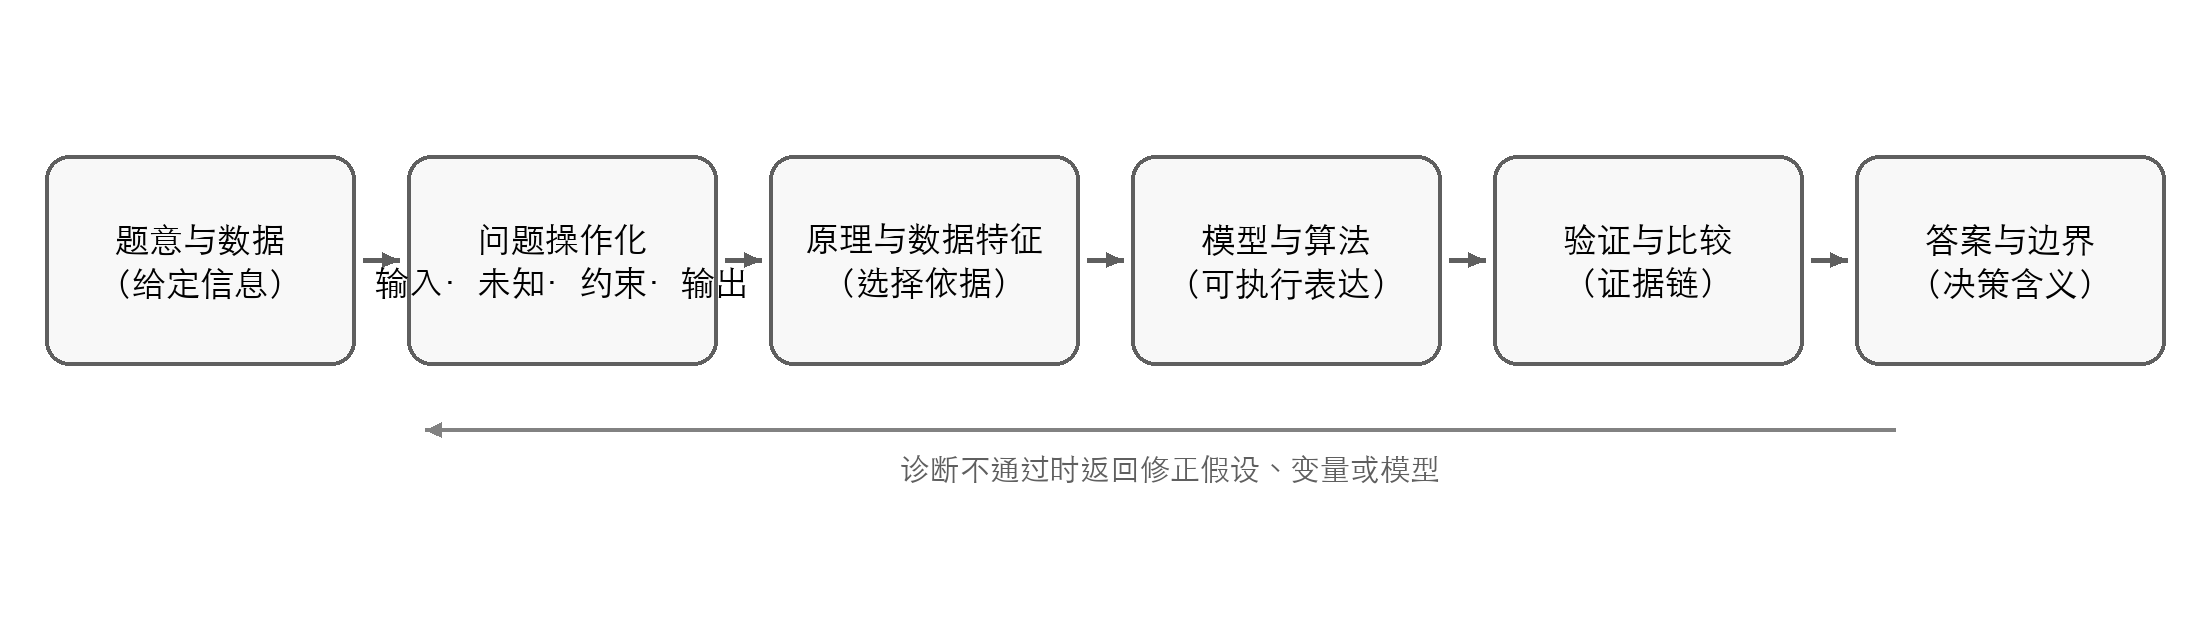
\includegraphics[width=0.96\textwidth]{figures/workflow.png}
  \caption{通用建模与证据闭环（按本题实际步骤替换括号内容）}
\end{figure}

\section{模型假设与符号说明}

\subsection{建模假设}

\textbf{假设1：}\fillin{填写被理想化的对象或过程}。依据是\fillin{题目信息、尺度分析或数据证据}；它使\fillin{被消去的自由度或简化的关系}成为可能。若\fillin{失效条件}发生，则预计会使结果\fillin{说明偏差方向或影响环节}。

\textbf{假设2：}\fillin{填写随机性、独立性、平稳性、均匀性或边界条件等假设}。采用它是因为\fillin{填写可检验理由}，并将在\fillin{填写诊断、灵敏度或对照实验}中检查其影响。

\textbf{假设3：}\fillin{填写决策时可获得的信息、参数恒定区间或约束可执行性}。该假设只适用于\fillin{填写时空范围或对象范围}，超出范围时需改用\fillin{填写可执行的扩展方向}。

\subsection{符号说明}

\begin{table}[htbp]
  \centering
  \caption{主要符号、单位与用途（按首次出现顺序增删）}
  \small
  \begin{tabularx}{0.94\textwidth}{C{1.8cm}LC{3.1cm}C{3.3cm}}
    \toprule
    符号 & 定义 & 单位或取值域 & 来源/首次用途 \\
    \midrule
    $x_i$ & \fillin{第$i$个样本或实体的输入} & \fillin{单位/集合} & \fillin{数据表/式号} \\
    $y_i$ & \fillin{对应的观测或响应} & \fillin{单位/集合} & \fillin{数据表/式号} \\
    $\bm\theta$ & \fillin{待估参数向量} & $\Theta$ & \fillin{式号} \\
    $\bm z_t$ & \fillin{时刻$t$的状态或隐变量} & \fillin{单位/集合} & \fillin{式号；静态任务可删除} \\
    $\bm u_t$ & \fillin{时刻$t$的决策变量} & $\mathcal U$ & \fillin{式号；无决策任务可删除} \\
    $J$ & \fillin{评价或目标函数} & \fillin{单位/无量纲} & \fillin{式号} \\
    $\varepsilon_i$ & \fillin{观测误差或未解释项} & \fillin{单位/分布} & \fillin{式号} \\
    \bottomrule
  \end{tabularx}
\end{table}

角度在三角函数、微分与程序内部统一使用弧度（$\mathrm{rad}$）；若题面或结果以度表示，只在输入与输出边界显式换算。倒数型单位写成$\mathrm{cm^{-1}}$等负指数形式。

\section{数据预处理与描述性统计（一般针对C题需要数据预处理的情形）}

\subsection{数据预处理}

\fillin{本章常见于需要清洗、整合和描述较大规模数据的C题，也适用于具有同类数据任务的A、B题；若数据量很小或没有预处理需求，可删除本章。先说明每个文件或数据表的粒度、主键、时空范围、单位与连接规则。}

\begin{table}[htbp]
  \centering
  \caption{数据质量审计与处理记录}
  \small
  \begin{tabularx}{0.96\textwidth}{C{1.6cm}LLL}
    \toprule
    检查项 & 观察到的证据 & 处理规则 & 可能影响 \\
    \midrule
    缺失 & \fillin{缺失比例、位置与是否成片} & \fillin{删除/插补/保留并建模} & \fillin{对样本量或偏差的影响} \\
    异常 & \fillin{物理越界、统计离群或录入错误} & \fillin{判据及阈值来源} & \fillin{对参数和结论的影响} \\
    重复 & \fillin{重复键、重复测量或重复事件} & \fillin{去重或聚合规则} & \fillin{对权重的影响} \\
    尺度 & \fillin{量纲差异、偏态、长尾或数量级} & \fillin{单位统一/变换/标准化} & \fillin{对数值稳定性的影响} \\
    依赖 & \fillin{时间、空间、分组或网络相关} & \fillin{分层/分块/留组验证} & \fillin{对不确定性的影响} \\
    \bottomrule
  \end{tabularx}
\end{table}

\subsection{描述性统计分析}

\fillin{分别报告关键变量的样本量、集中趋势、离散程度、取值范围和分布形态；再用时序图、分组图、相关图或空间图说明趋势、周期、偏态、异常点、组间差异和潜在关联。先陈述图表中能够直接观察到的事实，不在本节提前宣称因果关系或模型优劣。}

\begin{figure}[htbp]
  \centering
  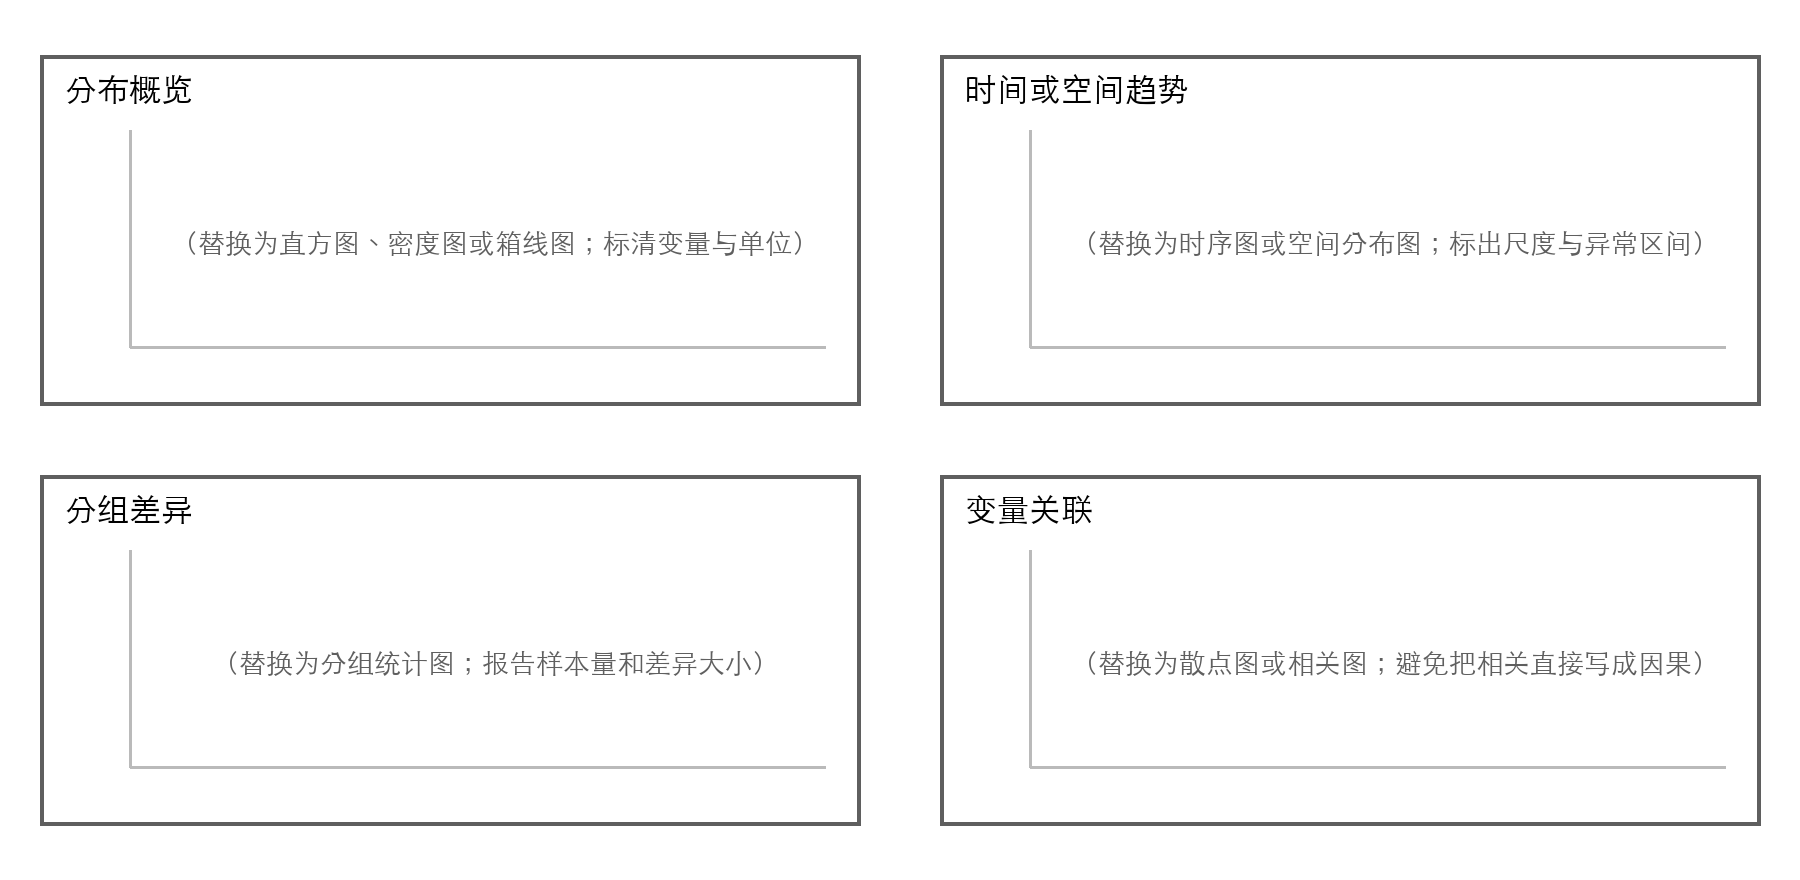
\includegraphics[width=0.90\textwidth]{figures/descriptive.png}
  \caption{描述性统计与数据特征图模板（只保留本题需要的面板）}
\end{figure}

\section{问题一建模与求解}

\subsection{问题一分析}

问题一要求\fillin{用一句话重述该问最终输出}。可重点说明\fillin{已知量与待求量之间尚缺少的关系、数据规律或决策冲突}。根据题型，可把研究对象表示为\fillin{实体、样本、区域、方案、指标或阶段}；若任务不涉及动态过程，无须引入状态或时间索引。

\subsubsection{问题一分析}

\begin{figure}[htbp]
  \centering
  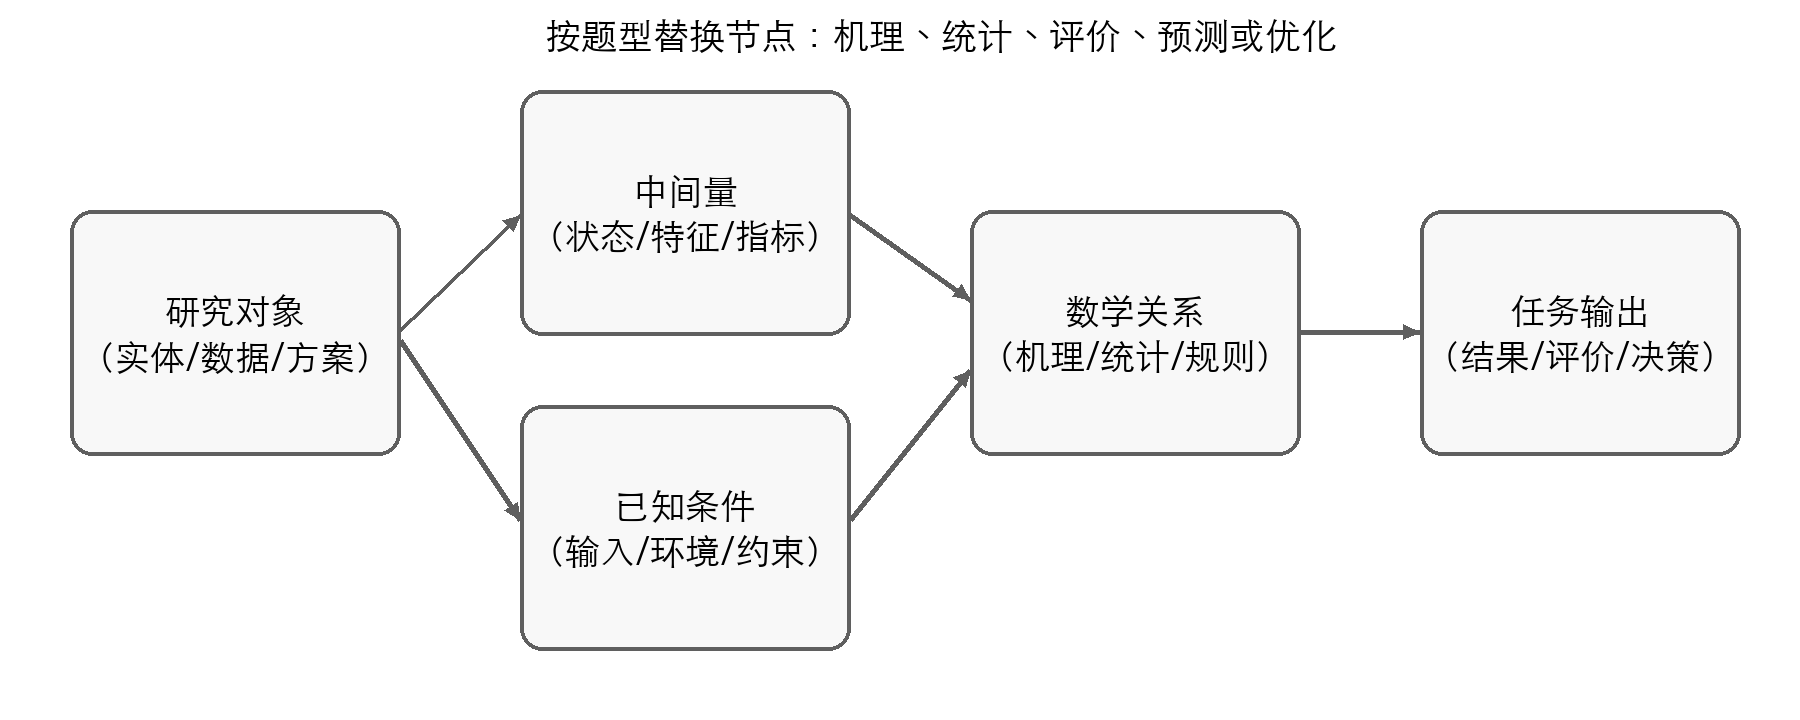
\includegraphics[width=0.90\textwidth]{figures/mechanism.png}
  \caption{问题一的关系结构与任务映射模板（按实际题型替换）}
\end{figure}

图中关系应按题型改写：机理题可填写“对象—状态—作用规律—观测”，统计或预测题可填写“数据—特征—估计/预测关系—输出”，评价或优化题可填写“方案—指标/决策—规则/约束—评分或方案”。

\subsubsection{问题一建模分析}

\fillin{若存在可手算、常识性规则或透明统计量，可先把它作为基准并说明覆盖范围；若没有合适基准，可直接从定义、题设关系或数据特征展开。正式模型增加的每一项均需对应题意或证据，并给出可检验的判断。}

\subsection{问题一建模}

\subsubsection{基础模型建模}

设\fillin{按本题需要定义对象或样本索引、坐标、参数、指标、决策量及其单位和取值域}。根据\fillin{守恒律、几何关系、概率定义、统计量、评价规则、收支平衡、效用原则或题设条款}，在\fillin{适用条件}下可写出通用隐式关系
\begin{equation}
  \mathcal G\!\left(\bm x,\bm\theta\right)=\bm 0.
\end{equation}
式中左端表示\fillin{填写物理或统计含义}，各项依次表示\fillin{逐项解释来源、符号和方向}。该式只在\fillin{边界、尺度或独立性条件}成立。

若式（1）含有不可直接计算的量，可消去\fillin{中间量}或引入\fillin{必要辅助量}；若原关系已可计算，则省略该步骤。一般的“输入—中间量—输出”结构可写为
\begin{equation}
  \bm z=\mathcal T(\bm x,\bm\theta),\qquad
  \bm y=\mathcal H(\bm z,\bm\theta)+\bm\varepsilon.
\end{equation}

\subsubsection{模型求解}

若任务涉及拟合、估计或预测，可定义
\begin{equation}
  \widehat y_i=f(\bm x_i;\bm\theta),\qquad
  r_i=y_i-\widehat y_i.
\end{equation}
其中$\bm x_i$为\fillin{输入}，$\bm\theta$为\fillin{待估参数及其范围}，$f$表示\fillin{映射}，$r_i$的单位与\fillin{观测量}一致。对解析计算、评价或确定性优化任务，应删除该式并改写为实际计算值、评分或目标量。

\subsubsection{模型分析}

若任务需要参数估计、方案优化或带权评价，可根据\fillin{异常点、异方差、偏好、离散选择或约束边界}写成
\begin{equation}
  (\widehat{\bm\theta},\widehat{\bm z})
  =\underset{\bm\theta\in\Theta,\,\bm z\in\mathcal Z}{\operatorname{arg\,min}}
  \left\{
  \sum_{i=1}^{n}w_i\rho\!\left(
  \frac{r_i(\bm\theta,\bm z)}{s_i}
  \right)+\lambda P(\bm\theta,\bm z)
  \right\}.
\end{equation}
式中$w_i$用于\fillin{说明权重来源}，$s_i$用于\fillin{说明尺度统一}，$\rho$用于\fillin{说明希望抑制或强调的误差}，$P$用于\fillin{说明复杂度或结构约束}。若本题只需解析求值、规则判断或直接统计，则删除该优化式。

\subsection{问题一建模与求解}

至此，根据题型把问题一归纳为以下一种或数种任务：计算\fillin{未知量}、估计\fillin{参数}、预测\fillin{响应}、评价\fillin{对象}或优化\fillin{决策}。仅在存在优化目标时使用“最优”和约束表述。

\begin{algorithmtable}{算法 1\quad 问题一求解伪代码（每一行应能追溯到公式或题意）}{可复用算法骨架}
1 & 输入：\fillin{数据、常数、参数域、误差阈值与随机种子} \\
2 & 校验：\fillin{单位、范围、缺失、主键与约束一致性} \\
3 & 初始化：\fillin{参数/状态/候选解及其来源} \\
4 & 对\fillin{样本、时刻、区域或候选方案}逐一执行 \\
5 & 按本题保留的公式或规则计算\fillin{中间量与任务结果} \\
6 & 若\fillin{精确判定条件}成立，则\fillin{分支更新}；否则\fillin{另一分支} \\
7 & 计算\fillin{误差、得分、守恒偏差、约束违背量或其他证据} \\
8 & 若使用迭代算法，则依据\fillin{更新规则}得到新解；否则记录结果 \\
9 & 若迭代任务达到\fillin{停止准则}则退出；否则继续下一对象 \\
10 & 返回：\fillin{答案、单位、不确定性、可行裕度与诊断结果} \\
\end{algorithmtable}

\subsection{问题一结果分析}

在\fillin{填写软件、版本、硬件或随机种子}下运行上述流程，得到\fillin{先用一句话回答问题一}。

\begin{table}[htbp]
  \centering
  \caption{问题一核心结果（表题应能说明对象、指标与条件）}
  \small
  \begin{tabularx}{0.96\textwidth}{YYYYY}
    \toprule
    方案/对象 & 主要结果（单位） & 不确定性/误差 & 约束裕度（可选） & 相对基准（可选） \\
    \midrule
    \fillin{对象A} & \fillin{数值＋单位} & \fillin{区间/误差} & \fillin{可选：最小裕度} & \fillin{可选：改善百分比} \\
    \fillin{对象B} & \fillin{数值＋单位} & \fillin{区间/误差} & \fillin{可选：最小裕度} & \fillin{可选：改善百分比} \\
    \fillin{推荐方案} & \fillin{数值＋单位} & \fillin{区间/误差} & \fillin{可选：最小裕度} & \fillin{可选：选择理由} \\
    \bottomrule
  \end{tabularx}
\end{table}

表中\fillin{可直接核验的数值、排序或差异}支持\fillin{对原问的回答}，可由式\fillin{式号}中的\fillin{主导项或规则}解释。仅在适用时保留约束裕度和相对基准两列。

\subsection{问题一稳定性与灵敏度分析}

根据题型选择验证：机理或几何模型检查量纲、守恒和极端情形；统计或预测模型检查拟合、残差和留出误差；评价模型检查权重与排序稳定性；优化模型检查可行性、基准比较和扰动稳定性。

\begin{figure}[htbp]
  \centering
  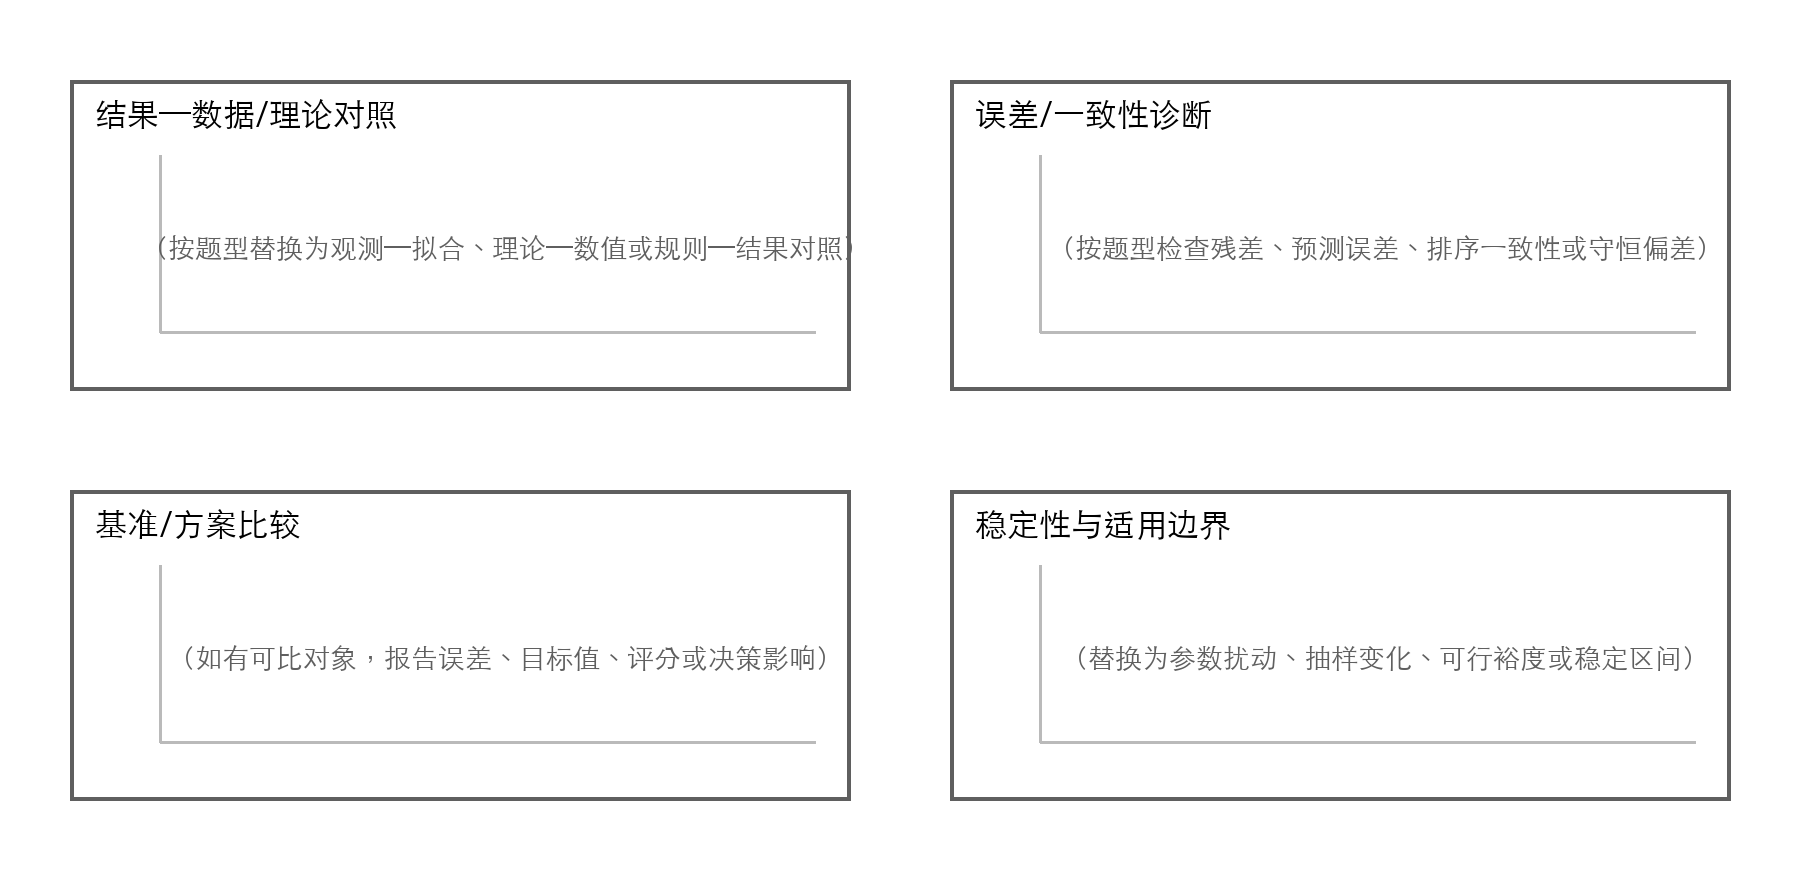
\includegraphics[width=0.90\textwidth]{figures/evidence.png}
  \caption{问题一结果证据图模板（只保留适用面板）}
\end{figure}

\section{问题二建模与求解}

\subsection{问题二分析}

先判断问题二与问题一的关系：若问题二沿用前问结果，说明新增的未知量、条件、评价要求或决策；若两问相对独立，则分别建立模型，不必人为继承问题一。本问要求输出\fillin{最终答案}，可复用的量为\fillin{已验证关系、数据处理或参数}，仍需解决的是\fillin{新增困难}。

\begin{table}[htbp]
  \centering
  \caption{问题二模型扩展的证据—结构对应关系}
  \small
  \begin{tabularx}{0.94\textwidth}{LLLL}
    \toprule
    观察证据 & 若忽略会怎样 & 需要的模型结构 & 如何检验 \\
    \midrule
    \fillin{数据特征1} & \fillin{残差/偏差/不可行} & \fillin{新增状态、项或约束} & \fillin{诊断图或统计量} \\
    \fillin{数据特征2} & \fillin{残差/偏差/不可行} & \fillin{新增状态、项或约束} & \fillin{诊断图或统计量} \\
    \fillin{边界或规则} & \fillin{产生不合法解} & \fillin{硬约束或分支判据} & \fillin{可行率/裕度} \\
    \bottomrule
  \end{tabularx}
\end{table}

\subsubsection{任务分析}

\fillin{若本问是参数反演或状态估计，解释观测如何识别未知量、误差为何采用相应损失；若本问是预测，说明训练信息截止时刻、验证切分和多步误差；若本问是优化决策，先写决策变量、目标、硬约束和不确定性，再选择求解算法。删除不适用的说明。}

\subsubsection{问题二建模分析}

\begin{figure}[htbp]
  \centering
  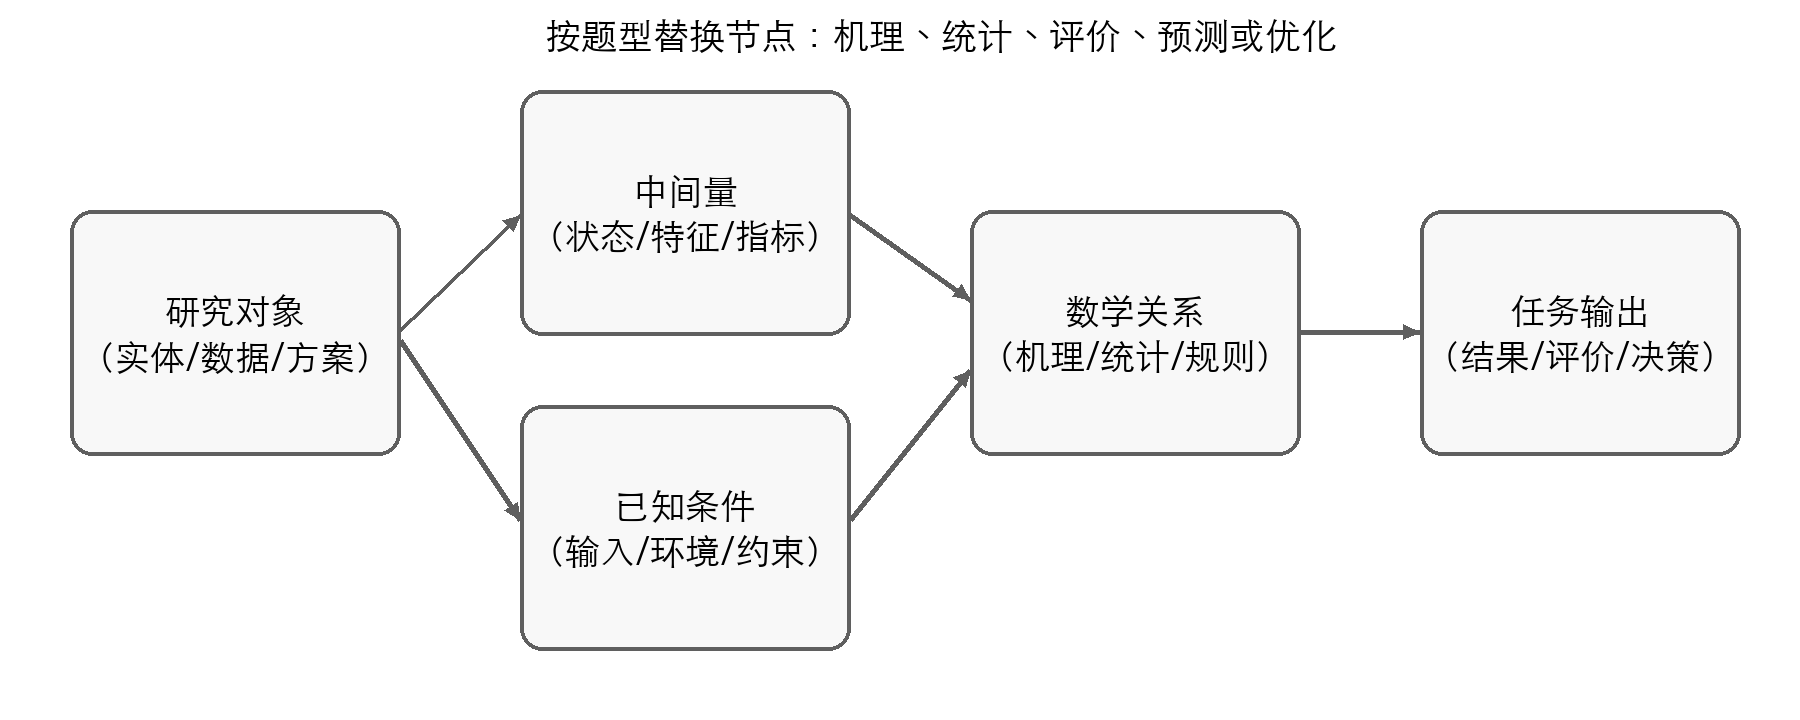
\includegraphics[width=0.88\textwidth]{figures/mechanism.png}
  \caption{问题二的新增关系/信息流（用本问实际对象重绘）}
\end{figure}

\subsection{问题二建模}

\subsubsection{变量分析}

若需要新增变量，可定义
\begin{equation}
  \bm g=\mathcal T(\bm x;\bm\eta).
\end{equation}
在数据题中$\bm g$可表示特征，在评价题中可表示标准化指标，在机理题中可表示辅助量，只有动态或序列任务才扩展为带时间下标的状态递推。若无需新增变量，删除式（5）。

\subsubsection{模型建立}

若题目要求估计、评价或优化，可将误差、得分、效益、风险或综合代价统一到可比尺度，写成
\begin{equation}
  J(\bm u,\bm\theta,\bm z)
  =J_{\mathrm{main}}
  +\lambda_{\mathrm{risk}}J_{\mathrm{risk}}
  +\lambda_{\mathrm{reg}}P.
\end{equation}
对纯机理计算或规则判定，应删除式（6）并保留实际计算关系。若存在约束，按实际来源列出物理、资源、容量、几何、时间、顺序、逻辑或变量边界。

\subsubsection{模型分析}

对估计或优化任务，可写成
\begin{equation}
  (\widehat{\bm u},\widehat{\bm\theta},\widehat{\bm z})
  =\underset{\bm u\in\mathcal U,\,\bm\theta\in\Theta,\,\bm z\in\mathcal Z}
  {\operatorname{arg\,min}}J(\bm u,\bm\theta,\bm z),
  \qquad
  \mathrm{s.t.}\quad h_k=0,\quad q_{\ell}\le 0.
\end{equation}
若本问是预测、评价、分类或解析计算，删除式（7），改写为对应的预测函数、评分规则、分类判据或计算式。

\subsection{问题二结果分析}

根据本问的计算结构选择方法：估计或优化任务说明连续/离散、凸/非凸、可微/黑箱和规模；预测任务说明训练、验证和推断流程；评价任务说明标准化、权重和合成规则；机理或几何任务说明数值计算与分支处理。

\begin{algorithmtable}{算法 2\quad 问题二求解伪代码}{步骤}
1 & 输入：\fillin{问题一输出、新增数据、变量域、约束、容差和种子} \\
2 & 构造：按式（5）生成\fillin{新增状态/变换}，并检查定义域 \\
3 & 初始化：\fillin{可行解或参数；记录初始目标和约束裕度} \\
4 & 循环直到\fillin{明确停止准则} \\
5 & 计算式（6）的各目标分量及式（7）的约束违背量 \\
6 & 若\fillin{分支/可行判据}成立，则\fillin{更新}；否则\fillin{修复或拒绝} \\
7 & 与当前候选解比较并保存\fillin{目标、状态、诊断} \\
8 & 结束循环；对所选候选执行\fillin{独立复核或精细计算} \\
9 & 返回：\fillin{方案、目标值、可行裕度、不确定性和对照结果} \\
\end{algorithmtable}

\begin{table}[htbp]
  \centering
  \caption{问题二结果与基准比较}
  \small
  \begin{tabularx}{0.96\textwidth}{YYYYYY}
    \toprule
    方法/方案 & 主要目标（单位） & 误差或风险 & 可行裕度 & 计算代价 & 结论 \\
    \midrule
    \fillin{透明基准} & \fillin{数值} & \fillin{数值} & \fillin{数值} & \fillin{时间/次数} & \fillin{基准表现} \\
    \fillin{所选方法} & \fillin{数值} & \fillin{数值} & \fillin{数值} & \fillin{时间/次数} & \fillin{改善及代价} \\
    \fillin{备选方法} & \fillin{数值} & \fillin{数值} & \fillin{数值} & \fillin{时间/次数} & \fillin{为何不选} \\
    \bottomrule
  \end{tabularx}
\end{table}

\subsection{问题二稳定性与灵敏度分析}

\begin{figure}[htbp]
  \centering
  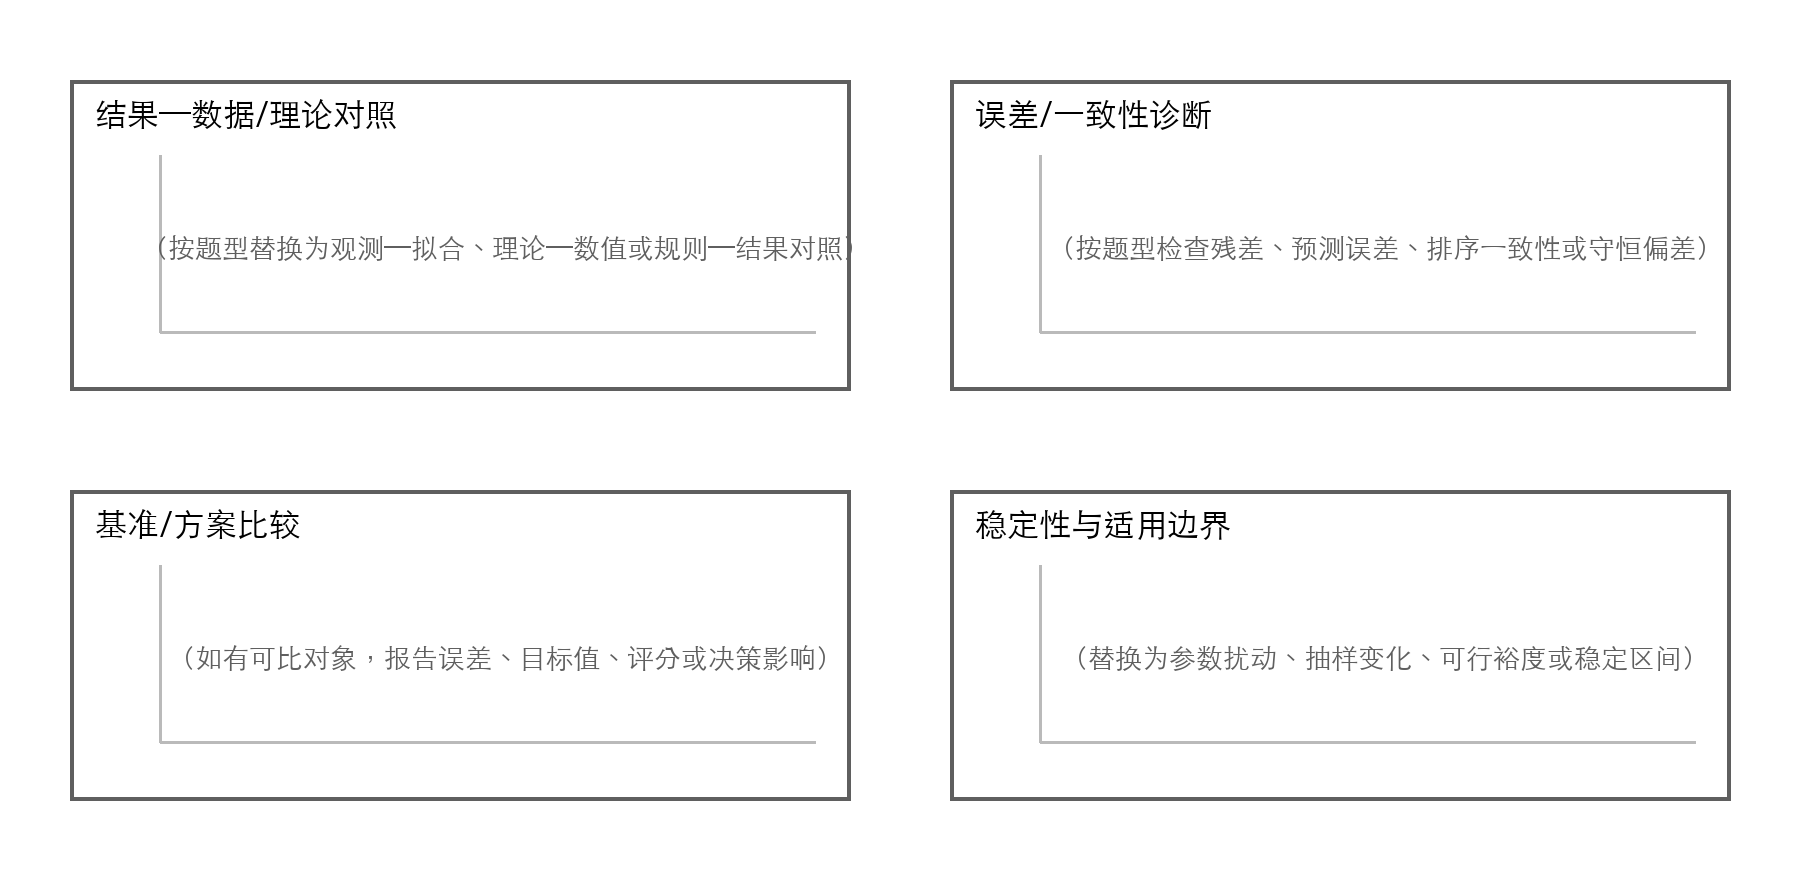
\includegraphics[width=0.86\textwidth]{figures/evidence.png}
  \caption{问题二的结果证据与对照模板（只保留适用面板）}
\end{figure}

图表共同表明\fillin{先报告可直接核验的数值或图形事实}。若设置了基准，比较绝对差异和相对变化；若没有合理基准，则报告误差、判据、一致性、可行性或稳定区间。

\section{问题三建模与求解}

\subsection{问题三分析}

问题三要求\fillin{最终输出}。先判断它是前两问的扩展、综合应用，还是相对独立的新任务。根据题型选择表示方式：机理或网络任务可定义实体、接口和作用关系；统计或预测任务可定义样本、特征和响应；评价任务可定义对象、指标和权重；优化任务可定义决策、目标与约束。

\subsubsection{问题三建模分析}

\begin{figure}[htbp]
  \centering
  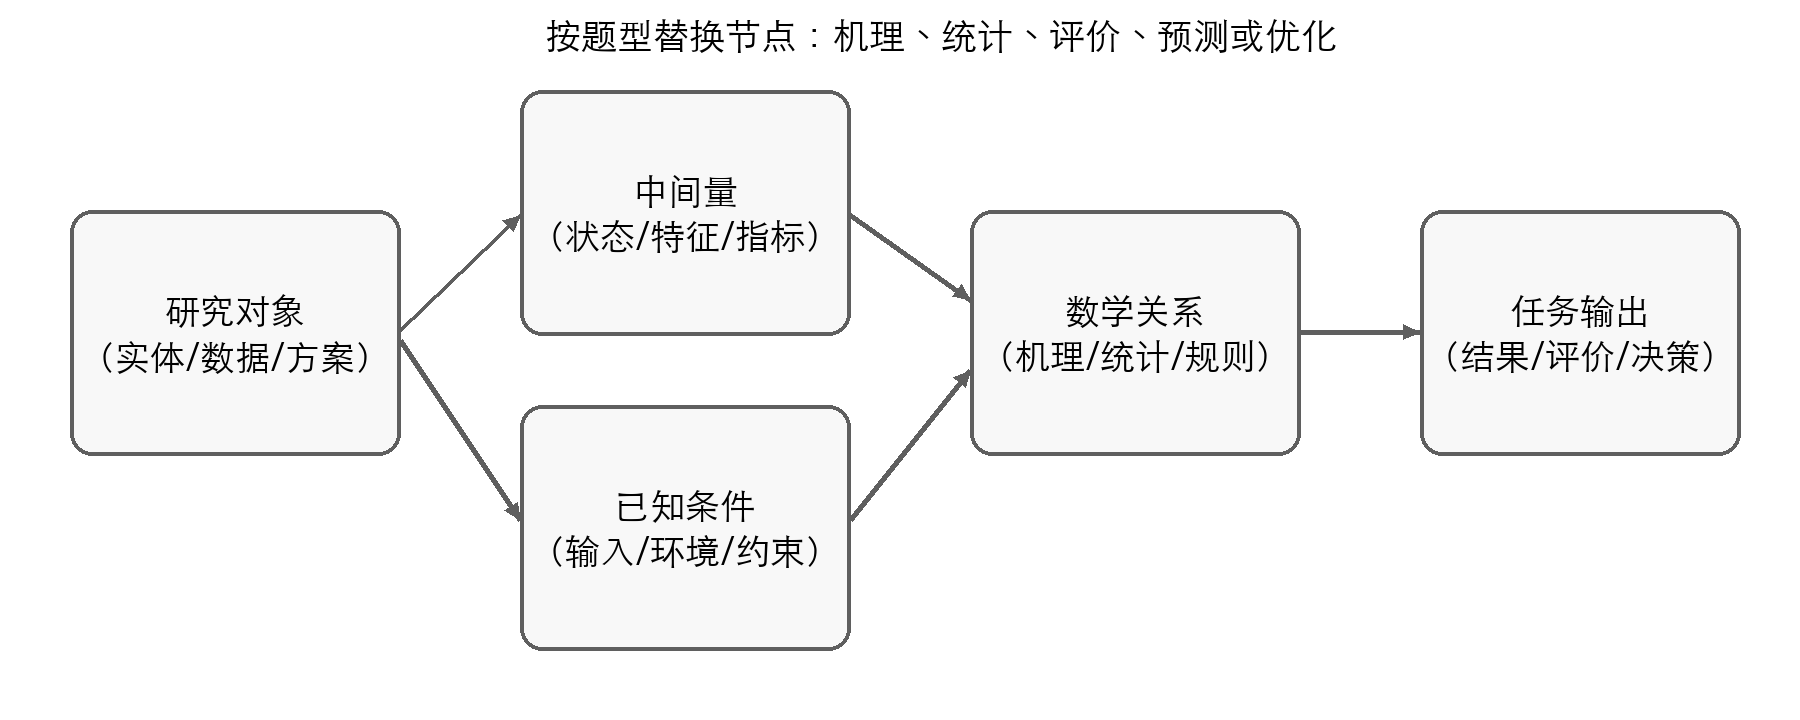
\includegraphics[width=0.90\textwidth]{figures/mechanism.png}
  \caption{问题三关系结构图模板（按实际题型替换节点与箭头）}
\end{figure}

\subsubsection{模型分析}

\begin{table}[htbp]
  \centering
  \caption{问题三模型结构增量分析}
  \small
  \begin{tabularx}{0.94\textwidth}{YLLYY}
    \toprule
    新增结构 & 对应的题意/数据证据 & 增加的参数或计算 & 是否改变答案 & 保留结论 \\
    \midrule
    \fillin{耦合项} & \fillin{证据} & \fillin{数量/代价} & \fillin{改变程度} & \fillin{保留/删除} \\
    \fillin{分支变量} & \fillin{证据} & \fillin{数量/代价} & \fillin{改变程度} & \fillin{保留/删除} \\
    \fillin{随机/鲁棒项} & \fillin{证据} & \fillin{数量/代价} & \fillin{改变程度} & \fillin{保留/删除} \\
    \bottomrule
  \end{tabularx}
\end{table}

\subsection{问题三建模}

若本问涉及动态、序列、空间相邻、层级传递或网络传播，可对\fillin{对象或节点索引}在\fillin{时间、空间或层级索引}下定义状态/中间量，并写成
\begin{equation}
  \bm z_{t+1}=F_t(\bm z_t,\bm x_t,\bm u_t).
\end{equation}
若本问是静态统计、评价、分类、几何计算或一般优化，则删除该递推式，改写为实际的估计式、评分式、判别式、几何关系或约束关系。

仅在需要多对象、多时期或多指标聚合时保留下式：
\begin{equation}
  Y=\sum_{j\in\mathcal J}\sum_{t\in\mathcal T}
  \omega_{jt}H_{jt}(\bm z_{jt},\bm u_{jt}).
\end{equation}
说明权重来源、重复计算和归一化规则；若输出由单一关系直接得到，则删除式（9）。

\subsection{问题三结果分析}

采用\fillin{与本问类型相符的计算、估计、预测、评价或优化流程}，生成主要结果并执行相应复核。

\begin{table}[htbp]
  \centering
  \caption{问题三结果与证据}
  \small
  \begin{tabularx}{0.96\textwidth}{YYYYYY}
    \toprule
    对象/情形/方案 & 主要结果（单位） & 误差/不确定性 & 约束或判据（可选） & 对照结果（可选） & 结论 \\
    \midrule
    \fillin{对象/情形1} & \fillin{数值} & \fillin{区间/误差} & \fillin{裕度/判据} & \fillin{差异} & \fillin{解释} \\
    \fillin{对象/情形2} & \fillin{数值} & \fillin{区间/误差} & \fillin{裕度/判据} & \fillin{差异} & \fillin{解释} \\
    \fillin{推荐结果} & \fillin{数值} & \fillin{区间/误差} & \fillin{裕度/判据} & \fillin{差异} & \fillin{解释} \\
    \bottomrule
  \end{tabularx}
\end{table}

\section{模型稳定性与灵敏度分析}

\subsection{稳定性分析}

验证可从低成本、强约束的检查开始，再进入与本题任务相符的数据或决策验证。根据题型选择：量纲与符号；可手算/退化情形；理论恒等式或守恒关系；拟合、残差或预测误差；排序或评价一致性；可行性与基准比较；输入扰动和外推边界。

\begin{table}[htbp]
  \centering
  \caption{模型验证证据账本}
  \small
  \begin{tabularx}{0.94\textwidth}{C{1.4cm}LLYL}
    \toprule
    层级 & 验证对象 & 判据 & 结果 & 失败时动作 \\
    \midrule
    结构 & \fillin{量纲、符号、索引、边界} & \fillin{理论恒等/范围} & \fillin{通过/数值} & \fillin{返回修正定义} \\
    数值 & \fillin{收敛、容差、随机性} & \fillin{误差阈值/重复稳定} & \fillin{通过/数值} & \fillin{加密/换初值/复算} \\
    数据 & \fillin{拟合、残差、留出样本} & \fillin{评价指标阈值} & \fillin{通过/数值} & \fillin{调整结构而非只调参} \\
    决策 & \fillin{可行性、排序、效益} & \fillin{裕度/基准改善} & \fillin{通过/数值} & \fillin{回退到保守方案} \\
    \bottomrule
  \end{tabularx}
\end{table}

\subsection{不确定性分析}

不确定性来自\fillin{测量误差、抽样波动、参数估计、模型结构、未来情景或数值误差}。其中\fillin{主导来源}通过式\fillin{式号}的\fillin{具体项}传播到最终答案。采用\fillin{解析传播、重采样、情景扫描或区间计算}得到\fillin{置信区间、预测区间或最坏情形范围}。

\subsection{灵敏度分析}

在\fillin{扰动范围和情景集合}内，核心结论\fillin{保持/不保持}，推荐方案的\fillin{关键指标}变化不超过\fillin{阈值}。当\fillin{临界条件}发生时，方案排序或可行性改变，因此建议应写成“若\fillin{条件}，则\fillin{行动}；否则\fillin{备选}”，而非无条件断言。

\section{模型评价}

\subsection{模型优点分析}

\fillin{优点1：指出模型在哪一项关键任务上表现好，并引用对应的表/图/误差/约束裕度；随后说明这一优点来自哪个结构，而不是只写“精度高、实用性强”。}

\fillin{优点2：说明可解释性、计算效率、鲁棒性或可复现性中的一项，并给出基准比较或运行证据。}

\subsection{模型局限分析}

\begin{table}[htbp]
  \centering
  \caption{局限—影响—改进闭环}
  \small
  \begin{tabularx}{0.94\textwidth}{YLLLL}
    \toprule
    局限或假设 & 何时失效 & 偏差方向/影响对象 & 当前缓解 & 可执行改进 \\
    \midrule
    \fillin{局限1} & \fillin{条件/范围} & \fillin{高估/低估/不稳定} & \fillin{灵敏度/保守界} & \fillin{新增数据或结构} \\
    \fillin{局限2} & \fillin{条件/范围} & \fillin{高估/低估/不稳定} & \fillin{对照/情景分析} & \fillin{新增数据或结构} \\
    \fillin{局限3} & \fillin{条件/范围} & \fillin{高估/低估/不稳定} & \fillin{边界声明} & \fillin{算法或实验改进} \\
    \bottomrule
  \end{tabularx}
\end{table}

\subsection{模型推广分析}

短期改进可在不改变主体框架的情况下加入\fillin{更可靠的数据处理、约束、诊断或求解策略}，预计改善\fillin{指标}，代价是\fillin{数据或计算成本}。推广到\fillin{新场景}时，可以保留\fillin{不依赖场景的守恒、几何、概率、统计或优化结构}；对\fillin{场景相关参数}通常需要重新标定，并在外部验证获得支持后再在声明的适用域内沿用结论。

\subsection{摘要结果核验}

正文完成后返回首页：对每一问只保留“对象—决定性依据—模型—带单位结果—证据—边界”；删除正文没有证明的形容词和方法堆砌。摘要中的每个数值都应能在正文表格或图中找到。

\label{main-body-end}

\clearpage
\begin{thebibliography}{99}
  \bibitem{ref1} \fillin{作者}. \fillin{文献题名}[J]. \fillin{期刊名}, \fillin{年份}, \fillin{卷(期)}: \fillin{起止页码}.
  \bibitem{ref2} \fillin{作者}. \fillin{书名}[M]. \fillin{版次}. \fillin{出版地}: \fillin{出版社}, \fillin{年份}.
  \bibitem{ref3} \fillin{作者}. \fillin{报告或学位论文题名}[R/D]. \fillin{机构或学校}, \fillin{年份}.
  \bibitem{ref4} \fillin{机构或作者}. \fillin{标准、规则或网页标题}[EB/OL]. \fillin{发布日期}[\fillin{引用日期}]. \fillin{稳定链接}.
  \bibitem{ref5} \fillin{软件/算法作者}. \fillin{软件或文档名称，版本号}[CP/OL]. \fillin{年份}. \fillin{稳定链接}.
\end{thebibliography}

\clearpage
\appendix

\section{数据字典与复现说明}

\subsection{文件与字段}

\begin{table}[htbp]
  \centering
  \caption{输入/输出文件清单}
  \small
  \begin{tabularx}{0.94\textwidth}{YLLLY}
    \toprule
    文件 & 一行/一个对象代表 & 主键 & 关键字段与单位 & 产生方式 \\
    \midrule
    \fillin{输入文件1} & \fillin{粒度} & \fillin{主键} & \fillin{字段：单位} & \fillin{题目附件/预处理} \\
    \fillin{中间结果1} & \fillin{粒度} & \fillin{主键} & \fillin{字段：单位} & \fillin{脚本与函数} \\
    \fillin{最终结果1} & \fillin{粒度} & \fillin{主键} & \fillin{字段：单位} & \fillin{脚本与函数} \\
    \fillin{作图数据1} & \fillin{粒度} & \fillin{主键} & \fillin{字段：单位} & \fillin{保存路径} \\
    \bottomrule
  \end{tabularx}
\end{table}

\subsection{运行环境与复现步骤}

\begin{enumerate}[leftmargin=2em,itemsep=0pt,topsep=2pt]
  \item \fillin{环境：操作系统、语言及版本、主要依赖及版本、硬件信息；随机算法固定种子}。
  \item \fillin{目录：说明原始数据只读目录、预处理结果目录、模型结果目录、图表目录和论文引用结果文件}。
  \item \fillin{运行：从主入口命令启动；配置文件为指定路径；不依赖手工修改中间文件}。
  \item \fillin{校验：运行前检查文件哈希、字段和单位；运行后检查关键量、约束违背量和图表数据一致性}。
  \item \fillin{复现判据：填写允许的绝对/相对误差；随机算法重复指定次数后报告均值、标准差和最优/最差结果}。
\end{enumerate}

\subsection{公式—代码—结果追溯表}

\begin{table}[htbp]
  \centering
  \caption{关键计算链追溯}
  \small
  \begin{tabularx}{0.90\textwidth}{YYYYY}
    \toprule
    数学对象 & 公式 & 代码函数 & 输出字段 & 正文证据 \\
    \midrule
    \fillin{中间状态} & \fillin{式号} & \fillin{函数名} & \fillin{字段名} & \fillin{图/表号} \\
    \fillin{目标/损失} & \fillin{式号} & \fillin{函数名} & \fillin{字段名} & \fillin{图/表号} \\
    \fillin{约束} & \fillin{式号} & \fillin{函数名} & \fillin{字段名} & \fillin{图/表号} \\
    \fillin{最终答案} & \fillin{式号} & \fillin{函数名} & \fillin{字段名} & \fillin{图/表号} \\
    \bottomrule
  \end{tabularx}
\end{table}

\clearpage
\section{完整算法与代码}

\fillin{正式提交时，本附录包含从读取数据到生成论文全部数值与图表的完整代码：配置、预处理、模型、目标、约束、求解、分支、验证、导出和主入口。不用截图、省略号或“其余同理”；下列骨架需用实际实现替换。}

\subsection{主程序与配置}

\begin{Verbatim}[fontsize=\scriptsize,breaklines=true,breakanywhere=true,frame=single]
from pathlib import Path

CONFIG = {
    "input_dir": Path("填写原始数据目录"),
    "output_dir": Path("填写结果目录"),
    "seed": 0,          # 填写随机种子
    "tolerance": 1e-8, # 填写收敛容差
    "max_iter": 1000,  # 填写最大迭代次数
}

def load_and_validate(config):
    """读取文件；检查字段、主键、单位、缺失、范围和哈希。"""
    raise NotImplementedError

def preprocess(raw, config):
    """实现数据质量审计表中的每一条处理规则。"""
    raise NotImplementedError
\end{Verbatim}

\subsection{模型、目标与约束}

\begin{Verbatim}[fontsize=\scriptsize,breaklines=true,breakanywhere=true,frame=single]
def model_map(data, parameters, state, config):
    """逐行对应正文公式或本题实际关系。"""
    raise NotImplementedError

def objective(candidate, data, config):
    """返回总目标及各分项；非优化任务删除本函数。"""
    raise NotImplementedError

def constraints(candidate, data, config):
    """返回每条约束值、裕度和可行标志。"""
    raise NotImplementedError

def solve(data, config):
    """实现初始化、循环、精确分支、停止准则和返回值。"""
    raise NotImplementedError
\end{Verbatim}

\clearpage
\subsection{验证、导出与主入口}

\begin{Verbatim}[fontsize=\scriptsize,breaklines=true,breakanywhere=true,frame=single]
def verify(data, solution, config):
    """执行量纲、极端情形、残差、基准、灵敏度或约束验证。"""
    raise NotImplementedError

def export_results(data, solution, diagnostics, config):
    """导出正文表格数据、作图数据、图像和复现清单。"""
    raise NotImplementedError

def main():
    raw = load_and_validate(CONFIG)
    data = preprocess(raw, CONFIG)
    solution = solve(data, CONFIG)
    diagnostics = verify(data, solution, CONFIG)
    export_results(data, solution, diagnostics, CONFIG)
    return solution, diagnostics

if __name__ == "__main__":
    main()
\end{Verbatim}

\subsection{提交前自检清单}

\begin{enumerate}[leftmargin=2em,itemsep=0pt,topsep=2pt]
  \item \fillin{所有待填括号已替换，没有留下教学提示语}。
  \item \fillin{每个摘要数值均能追溯到正文图表、公式和代码输出}。
  \item \fillin{单位、角度、坐标、符号、有效数字和误差口径全文一致}。
  \item \fillin{文中引用与参考文献一一对应；赛题附件不作为普通参考文献}。
  \item \fillin{完整代码可从主入口独立运行，并能重生正文全部结果与图表}。
\end{enumerate}

\end{document}
